%NYU 2019 Grad Computational Physics Homework 5

\documentclass[12pt, graphicx]{article}
\pagestyle{plain}
\baselineskip 18pt
\textwidth 6.5in
\textheight 7.8in
\oddsidemargin 0.1in
\evensidemargin 0.1in
\topmargin 0.3in
\parindent 0pt
\linespread{1.5}
\setlength{\parskip}{2.5mm}

\usepackage{graphicx, psfrag, epsfig}
\usepackage[font = small, format = plain, labelfont = bf, textfont = it, justification = raggedright, singlelinecheck = false]{caption}
\usepackage{subfig}
\usepackage{amsmath, amssymb}
\usepackage{geometry}
%\usepackage[symbol]{footmisc}

\renewcommand\tablename{Table}
\renewcommand\figurename{Fig.}
\renewcommand{\thefootnote}{\fnsymbol{footnote}}


\begin{document}
\title{Computational Physics Homework 5}
\author{Hao Li\footnotemark[2]}
\footnotetext[2]{hl3270@nyu.edu~~UID:N12137527}
\date{\today}


\maketitle

\section*{Problem 1}
\subsection*{a)}
Origional ODE:
\begin{equation}
\frac{\mathrm{d}^2x}{\mathrm{d}t^2}=-g
\end{equation}
Now replace the second derivative with:
\begin{equation}
x''(t)=\frac{x(t+h)-2x(t)+x(t-h)}{h^2}
\end{equation}
Put $x(t)$ on the left side and others on the right, and we will get the relaxation method equation:
\begin{equation}
x^*(t)=\frac{1}{2}[x(t-h)+x(t+h)]+\frac{1}{2}gh^2
\label{eq:rel1}
\end{equation}

\subsection*{b)}
The code for calculating the boundary value problem with equation above and boundary values $x(0)=x(10)=0$ is available in \textquotedblleft iteration.h\textquotedblright, attached in the folder.\par

\begin{figure}[ht]
\centering
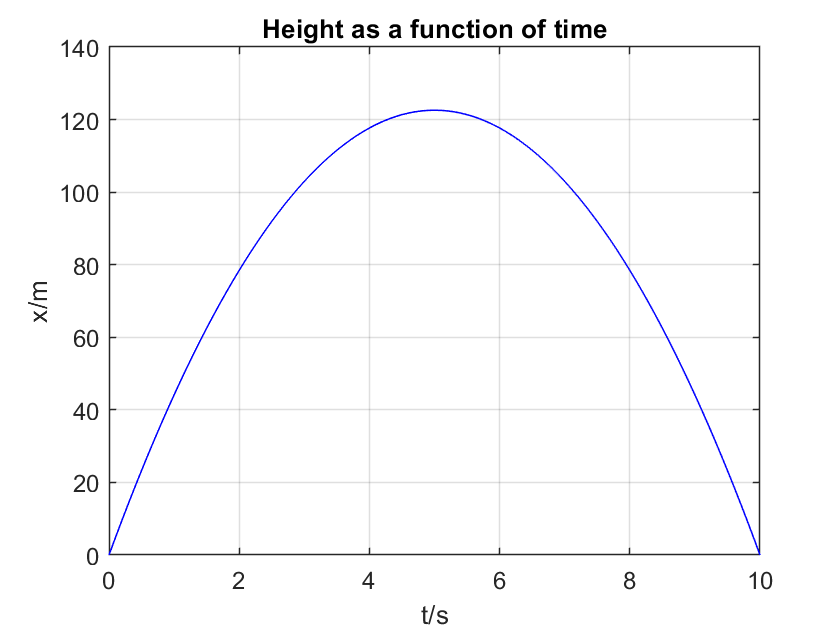
\includegraphics[width = 120mm]{trajectory.png}
\caption{The trajectory of a ball calculated by one dimensional relaxation method. Boundary values $x(0)=x(10)=0$, number of time grid cells $n_\mathrm{cell}=100$, target maximum difference is set to be $10^{-6}$. The result agrees well with the parabolic trajectory it should be.}
\label{fig:trajectory}
\end{figure}

By inputing the boundary values $x_\mathrm{left}(t_\mathrm{left})$, $x_\mathrm{right}(t_\mathrm{right})$,the number of grid cells $n_\mathrm{cell}$, and the target maximum difference for all grid points between two steps $\mathrm{max\_dif\_tar}$, the code will iterate using relaxation method in 1D with the relaxation equation \ref{eq:rel1} above, saves and shows the final values for each grid point $x(t_\mathrm{i})$.\par
The plot for the given boundary value problem is as shown in Figure.\ref{fig:trajectory}, which obviously agrees with the parabolic trajectory it should be. The data for this plot is saved in \textquotedblleft relax\_1D\_trajectory.txt\textquotedblright.

\section*{Problem 2}
\subsection*{(a)}
The cloud-in-cell (CIC) technique: Devide the domain of definition into grid cells centerd by grid points, and draw cells of the same shape centered by particles or points. Add the volume of particle cells (the clouds of the particles) overlapped by a grid cell to the amound for that center point, as shown in Figure. \ref{fig:CIC}. After adding all the particles in this way, the amount distribution of grid cells shows the CIC approximate for particle density.\par

\begin{figure}[ht]
\centering
\includegraphics[width = 120mm]{cloud_in_cell.png}
\caption{Cloud in cell technique. This picture shows an example in two dimensions. After dividing the whole area into grids, attach a cloud of the same shape and size of grid cell to each particle, centered by itself. The volume (area) of the cloud overlapped by a grid cell is added to the amount of particles of that cell centered by a grid point. After adding all the weighted volume, we will get a cloud-in-cell approximation of the density field of particles.}
\label{fig:CIC}
\end{figure}

The code for CIC technique is available in \textquotedblleft particle\_density.h\textquotedblright attached in the folder. The image for the distribution and the charge density field of the particles $(x,y)$ given in \textquotedblleft particles.txt\textquotedblright (renamed for convenience) are respectively ahown in Figure. \ref{fig:charge} and \ref{fig:density}. The data for the charge density field using CIC technique is saved in \textquotedblleft particle\_density\_two\_dim\_CIC.txt\textquotedblright.

\begin{figure}[ht]
\centering
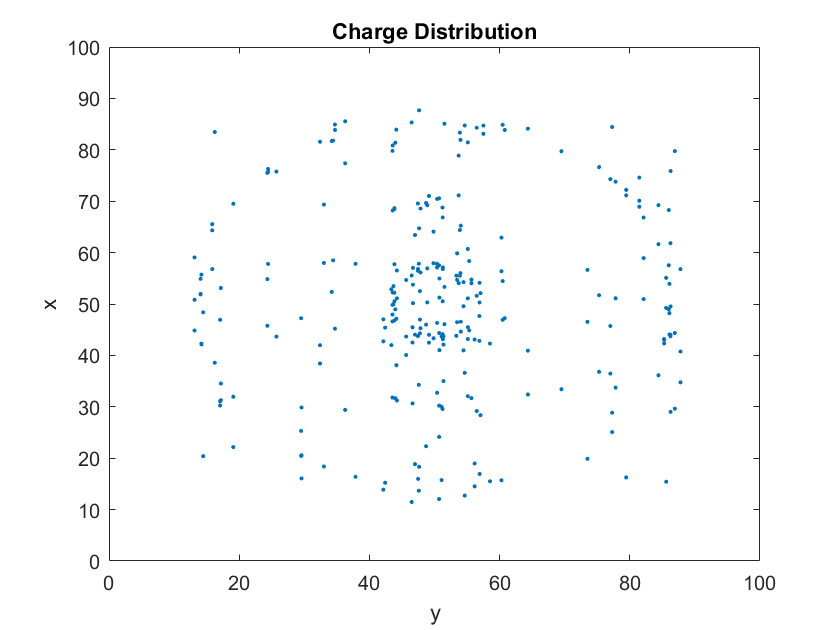
\includegraphics[width = 120mm]{charges.png}
\caption{The position distribution of particles in \textquotedblleft particles.txt\textquotedblright.}
\label{fig:charge}
\end{figure}

\clearpage

\begin{figure}[ht]
\centering
\includegraphics[width = 140mm]{charge_density.png}
\caption{The charge density field of particles in \textquotedblleft particles.txt\textquotedblright. The size of a grid cell is $1\times1$, with $100\times100$ grids. Each charge has the same charge $e$ as an electron.}
\label{fig:density}
\end{figure}

\subsection*{(b)}
Simmilar to Problem 1, in two dimensions, replace the Laplace operator with 
\begin{equation}
\begin{aligned}
\nabla^2\phi(x,y)&=\frac{\partial^2\phi(x,y)}{\partial x^2}+\frac{\partial^2\phi(x,y)}{\partial y^2}\\&=\frac{\phi(x+h_x,y)-2\phi(x,y)+\phi(x-h_x,y)}{h_x^2}+\frac{\phi(x,y+h_y)-2\phi(x,y)+\phi(x,y-h_y)}{h_y^2}
\end{aligned}
\label{eq:nabla}
\end{equation}
Here we use different size for x and y since they are not necessarily the same. Now plug Eq. \ref{eq:nabla} into Poisson's equation Eq. \ref{eq:Poisson} (in SI)
\begin{equation}
\nabla^2\phi=-\frac{\rho}{\epsilon_0}
\label{eq:Poisson}
\end{equation}
and then we will get a relaxation equation with $\phi(x,y)$ on the left side only, shown as Eq. \ref{eq:Poisson_rel} 
\begin{equation}
\begin{aligned}
\phi^*(x,y)=&\frac{h_y^2}{2(h_x^2+h_y^2)}[\phi(x+h_x,y)+\phi(x-h_x,y)]+\frac{h_x^2}{2(h_x^2+h_y^2)}[\phi(x,y+h_y)+\phi(x,y-h_y)]\\
&+\frac{h_x^2h_y^2}{2(h_x^2+h_y^2)}\frac{\rho(x,y)}{\epsilon_0}
\end{aligned}
\label{eq:Poisson_rel}
\end{equation}
In this subsection, we will use the standard relaxation method similar to Problem 1 using Eq. \ref{eq:Poisson_rel}, by refreshing $\phi(x_i,y_j)$ after an entire loop is finished. In this problem, all four sides are grounded so the boundary conditions are 
\begin{equation}
\phi(x=0)=\phi(x=100)=\phi(y=0)=\phi(y=100)=0
\label{eq:BC}
\end{equation}
The code for relaxation method to solve two dimensional boundary value problems is available in \textquotedblleft iteration.h\textquotedblright. By inputing the boundary of the box, the boundary conditions (if not simple, may input by function or file), number of grids for each side $n_x$, $n_y$, and the convergence criterion, i.e. the maximum difference for any cell in the grid between the current and prior step $\mathrm{max\_dif}$, the code will return the number of iterations, and the iteration result for each grid points, saved in a file. \par
In this problem, $x\in[0,100]$, $y\in[0,100]$, $n_x=M=100$, $n_y=M=100$, the boundary conditions are Eq.  \ref{eq:BC}, $\mathrm{max\_dif=1.0E-10}$, and $\rho(x,y)$ given by (a). \par
The image for the relaxation method result of the Poisoon's equation is shown in Figure. \ref{fig:pot_rel} and \ref{fig:pot_relc}. In Figure. \ref{fig:pot_relc} we can see clearly see the contour of potential goes from circular at the center to rectangular near boundary, agrees with our intuition. The data for this image is saved in \textquotedblleft relax\_2D\_potential.txt\textquotedblright. It takes 12056 iterations to converge to the target difference.

\begin{figure}[ht]
\centering
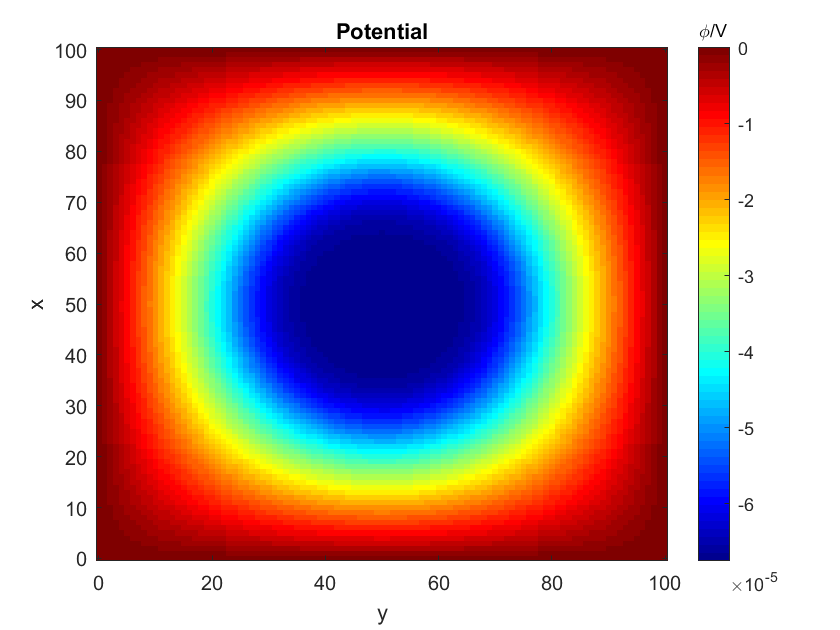
\includegraphics[width = 140mm]{potential.png}
\caption{The potential $\phi(x,y)$ for the charge density field of particles in \textquotedblleft particles.txt\textquotedblright, calculated using standard relaxation method.}
\label{fig:pot_rel}
\end{figure}

\clearpage

\begin{figure}[ht]
\centering
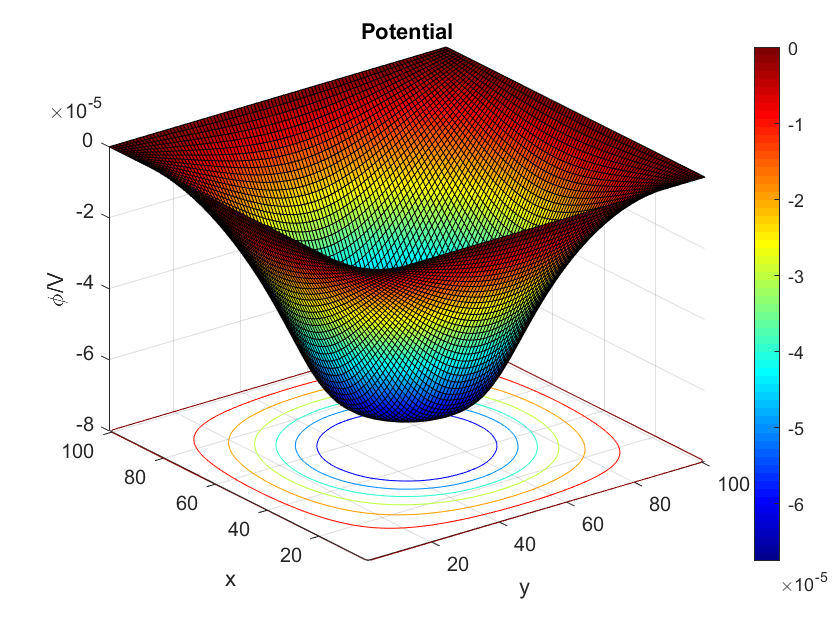
\includegraphics[width = 140mm]{potentialc.png}
\caption{The potential $\phi(x,y)$ for the charge density field of particles in \textquotedblleft particles.txt\textquotedblright, calculated using standard relaxation method, shown with contours of potential.}
\label{fig:pot_relc}
\end{figure}

\subsection*{(c)}
Similar to the standard relaxation method, Gauss-Seidel relaxation method refreshes the value at each point immediately when a new one is got. It does not ensure convergence, but sometimes this method is much faster than the standard one. The result of the same problem using Gauss-Seidel relaxation method is saved in \textquotedblleft GS\_relax\_2D\_potential.txt\textquotedblright, and it takes 6697 iterations to converge to the target difference, which is nearly twice faster than the standard method.\par
In this subsection, we use Gauss-Seidel overrelaxation method to solve the same Poisson's equation as in (b). Label the relaxation equation Eq. \ref{eq:Poisson_rel} as $\phi'(x,y)$, so the overrelaxation equation is 
\begin{equation}
\begin{aligned}
\phi_\omega(x,y)=&(1+\omega)\phi'(x,y)-\omega\phi(x,y)\\
=&\frac{(1+\omega)h_y^2}{2(h_x^2+h_y^2)}[\phi(x+h_x,y)+\phi(x-h_x,y)]+\frac{(1+\omega)h_x^2}{2(h_x^2+h_y^2)}[\phi(x,y+h_y)+\phi(x,y-h_y)]\\
&+\frac{(1+\omega)h_x^2h_y^2}{2(h_x^2+h_y^2)}\frac{\rho(x,y)}{\epsilon_0}+\omega\phi(x,y)
\end{aligned}
\end{equation}
For standard overrelaxation method, refresh $\phi(x,y)$ after a whole iteration, and for Gauss-Seidel overrelaxation method, refresh as soon as a new one is calculated. The range of parameter $\omega\in(-1,1)$. When $\omega=0$, it is the just the normal relaxation method. For $\omega\in(0,1)$, it is called overrelaxation method. For $\omega\in(-1,0)$, it is called underrelaxation method, which may not speed up calculation. When $\omega\to\pm1$, the calculation is instable. For some particular values of $\omega$, the number of iterations are significantly reduced, the best of which is the optimal value of the overrelaxation parameter $\omega_b$.\par
To find the optimal value of the parameter, we may use some root finding techniques, since the relationship of the number of iterations and the value of parameter is relatively smooth. Here golden ratio search is taken as an example. Firstly, for $\omega>0.985$, the calculation is too slow to tell if it could actually converge, so we choose the maximum of $\omega$for searching to be 0.984, and the minimum to be 0. Considering the slope of $n_\mathrm{iterations}(\omega)$, to get a clearer plot of it, the range is separated into two parts, [0, 0.981], and [0.98, 0.984]. Golden ratio search is used in the first part to get the optimal value parameter, and in the second for more details of the large slope part. Search stops when reaching the target precision, here is set to be 0.001.\par
The process of the golden ratio search is : \par
(1) Start with two boundaries $\omega_1$ and $\omega_4$. Calculate the two golden ratio points in the range $[\omega_1,\omega_4]$ : 
\begin{equation}
\begin{aligned}
\omega_2&=\omega_1+\frac{1+\sqrt{5}}{2}(\omega_4-\omega_1)=\frac{3-\sqrt{5}}{2}\omega_1+\frac{1+\sqrt{5}}{2}\omega_4\\
\omega_3&=\omega_4-\frac{1+\sqrt{5}}{2}(\omega_4-\omega_1)=\frac{1+\sqrt{5}}{2}\omega_1+\frac{3-\sqrt{5}}{2}\omega_4
\end{aligned}
\end{equation}
(2) Calculate the value of $n$ for each $\omega$, and find the minimum of these four $n$'s. \par
(3) If the minimum is at $\omega_1$ or $\omega_2$, then narrow the range of $\omega$ to $[\omega_1,\omega_3]$. So the new parameters
\begin{equation}
\begin{gathered}
\omega_4^*=\omega_3\\
\omega_3^*=\omega_2\\
\omega_2^*=\frac{3-\sqrt{5}}{2}\omega_1+\frac{1+\sqrt{5}}{2}\omega_4
\end{gathered}
\end{equation}
If the minimum is at $\omega_3$ or $\omega_4$, then narrow the range of $\omega$ to $[\omega_2,\omega_4]$. So the new parameters
\begin{equation}
\begin{gathered}
\omega_1^*=\omega_2\\
\omega_2^*=\omega_3\\
\omega_3^*=\frac{1+\sqrt{5}}{2}\omega_1+\frac{3-\sqrt{5}}{2}\omega_4
\end{gathered}
\end{equation}
(4) Calculate the value of $n$ for the new $\omega_2^*$ or $\omega_3^*$ added. \par
(5) Repete step (3) and (4) until reaching the target precision $\omega_4-\omega_1<\Delta\omega_\mathrm{tar}$\par

The data for these two calculations are saved in \textquotedblleft GS\_overrelax\_2D\_potential.txt\textquotedblright and \textquotedblleft GS\_overrelax\_2D\_potential(2).txt\textquotedblright. Figure. \ref{fig:iteration} shows the relationship of the number of iterations with the value of overrelaxation parameter $\omega$. In this figure, we can see that the number of iterations  drops gradually but significantly until reaching the optimal value $\omega_b\approx0.946$, and then explodes to infinity when reaching the instability point $\omega=1$. The optimal value of $\omega$ lies within [0.945,0.946]

\begin{figure}[ht]
\centering
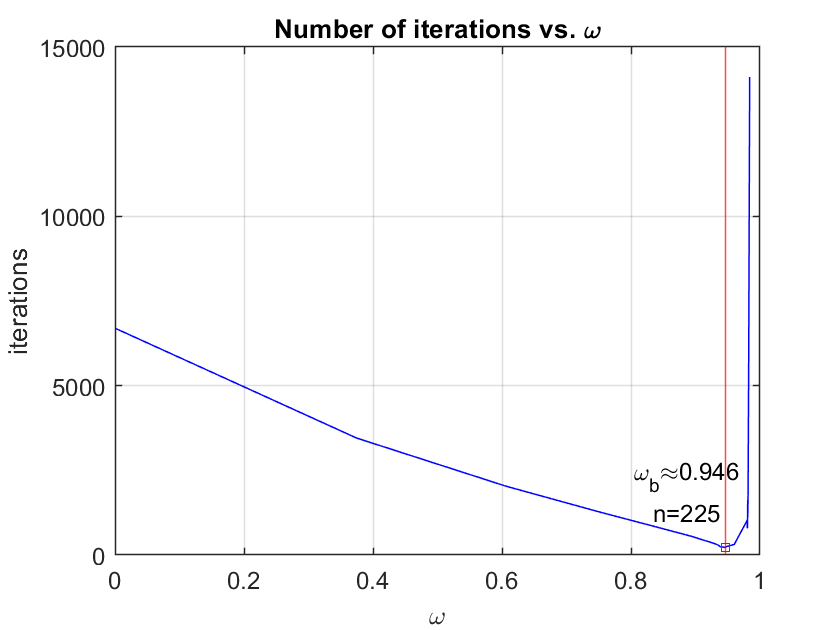
\includegraphics[width = 120mm]{iteration.png}
\caption{The relationship of the number of iterations with the value of overrelaxation parameter $\omega$, for the solution for Poisson's equation. As $\omega$ increases from 0 until reaching around $\omega_b\approx0.946$, the number of iterations decreases from arround 7000 to around 225. As it goes on increasing to 1, the number of iterations explodes to infinity.}
\label{fig:iteration}
\end{figure}

The evolution of $\omega$ with each step in the minimization process is shown in Figure. \ref{fig:golden}, while \ref{fig:golden1} shows the whole process, and \ref{fig:golden2} shows the details arround the final result. 

\begin{figure}[ht]
\subfloat[The whole minimization process.]{
\centering
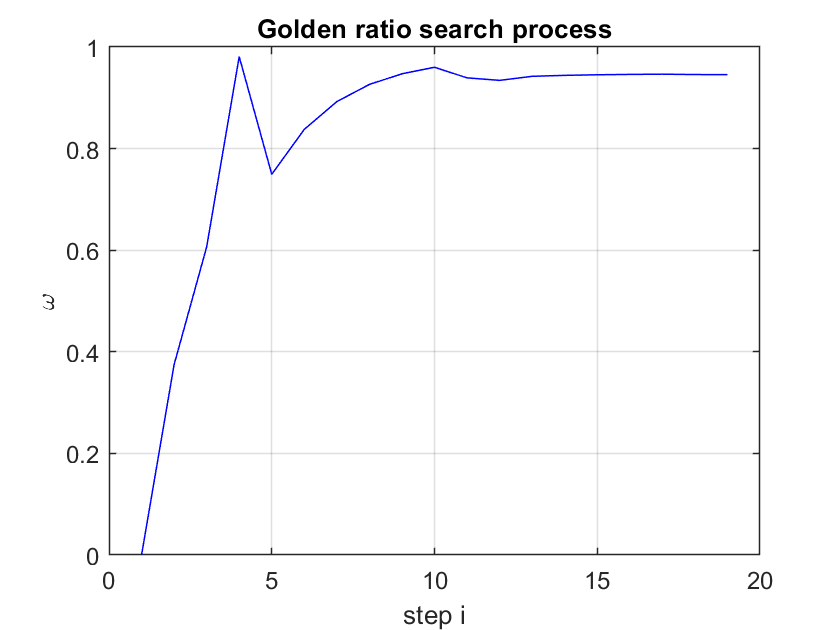
\includegraphics[width = 80mm]{golden_ratio.png}
\label{fig:golden1}
}
\subfloat[The detailed process when near the final answer.]{
\centering
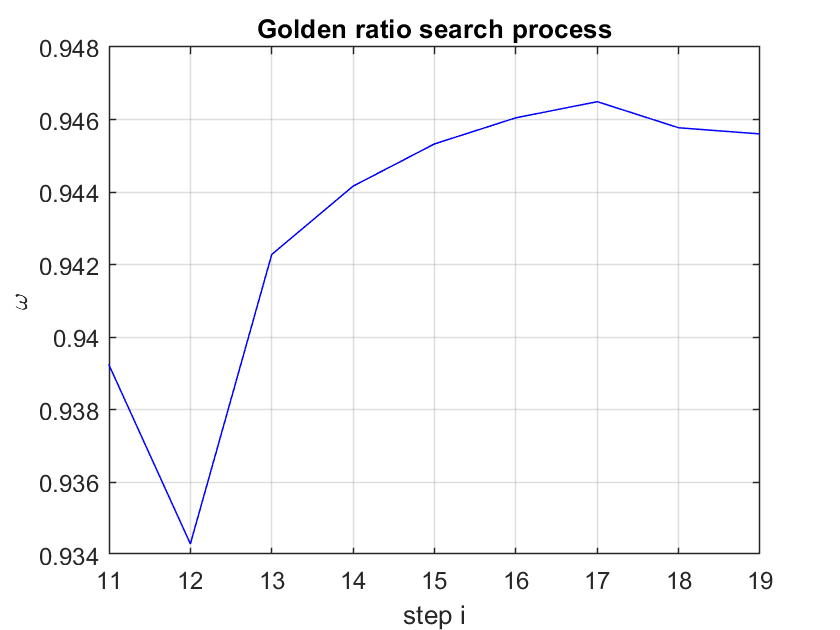
\includegraphics[width = 80mm]{golden_ratio_detailed.png}
\label{fig:golden2}
}
\caption{The evolution of the overrelaxation parameter $\omega$ with each step $\mathrm{i}$ in the minimization process. After arround ten steps, it reaches the vincinity of the optimal value of $\omega_b\approx0.946$}
\label{fig:golden}
\end{figure}




\end{document}